%---------------------- Set Document Commands -----------------------------

\documentclass[twocolumn,showpacs,preprintnumbers,amsmath,amssymb]{revtex4-1}

\usepackage{dsfont}
\usepackage{graphicx}% Include figure files
\usepackage{dcolumn}% Align table columns on decimal point
\usepackage{bm}% bold math
\usepackage{amsmath, amsthm, amssymb}
\usepackage{graphicx}
\usepackage{float}
\usepackage[spanish]{babel}
\usepackage[utf8]{inputenc}

%---------------------- End Document Commands ------------------------------
%---------------------------- Begin Document -------------------------------

\begin{document}

\renewcommand{\tablename}{Tabla}

%---------------------------------------------------------------------------
% TITLE SECTION
%---------------------------------------------------------------------------

\title{Efecto Hall, coeficiente de Hall de una punta de \textit{InAs} y su empleo para medir el campo magnético.}% Force line breaks with \\

\author{L. Felipe Gómez}
\email{L.Felipe_Gomez@ciencias.unam.mx}
\affiliation{Facultad de Ciencias, Universidad Nacional Autónoma de México}

\date{\today}

%---------------------------------------------------------------------------
% ABSTRACT SECTION
%---------------------------------------------------------------------------


\begin{abstract}

\begin{center}
\textbf{Resumen}
\end{center}

Utilizando el efecto Hall se caracteriza una punta Hall de InAs de dos formas distintas, a campo magnético externo constante y a corriente
de control constante, obteniendose un valor promedio de la constante de Hall de $R_H = (1.70 \pm 0.08)\times10^{-8} \frac{Vm}{AG}$, que determina el signo de los portadores
de carga del semiconductor. Se estudia la naturaleza vectorial del efecto Hall, observandose la variación del voltaje de
Hall conforme cambia el angúlo de incidencia del campo magnético externo. En la ultima parte utilizando la punta Hall
caracterizada, se mide el campo magnético tanto de un electroimán como de un imán en barra permanente, mostrándose los
resultados en mapas de calor que muestran la forma de su campo magnético.

\end{abstract}

\pacs{07.55.-w, 07.55.Ge}
\maketitle

%---------------------------------------------------------------------------
% THEORY SECTION
%---------------------------------------------------------------------------

\section{Introducción}

En 1879 Edwing Herbert Hall descurbio el efecto que lleva su nombre y recientemente en 1985 se descubrio el efecto Hall cuántico por Klaus
von Klitzing. En este experimento nos restringimos al efecto Hall clásico.

El efecto Hall es muy útil para estudir las propiedades eléctricas de los semiconductores, ya que permite conocer el
signo de los portadores de la carga y su concentración. Y un semiconductor caracterizado puede ser usado para medir campos
magnéticos.

En este experimento se busca caracterizar una punta Hall de InAs obteniendo su coeficiente de Hall, observar la naturaleza
vectorial del efecto Hall que se manifiesta como una dependencia del ángulo de la cara de la punta respecto a la dirección
campo magnético externo y la utilización del efecto Hall para medir el campo magnético de un electroimán y una barra iman
permanente.

El efecto Hall tiene presencia en un conductor o semiconductor por el que pasa una corriente $I_C$ y esta en presencia de un
campo magnético externo $B$. La interacción del campo magnético externo con el movimiento de los portadores de la carga produce
un reordenamiento de éstos en el material, debido a la fuerza de Lorentz, y se produce un nuevo campo eléctrico perpendicular
al campo magnético y al mismo campo eléctrico que produce la corriente. Al campo eléctrico producido se le conoce como \textit{campo
de Hall} que se denota como $E_H$.

\subsection{Efecto Hall Clásico}

El efecto Hall clásico[1] es una efecto producido por la fuerza de Lorentz (\textbf{Eq. 1}). En la \textbf{Fig. 1.} se muestra
un conductor o semiconductor por el que pasa una corriente de control $I$ a lo largo de éste. Hay un campo magnético $B$
que incide perpendicularmente. Suponiendo que los portadores de la carga tienen signo negativo se indica que se mueven en dirección
contraria. Por la fuerza de Lorentz habrá una acumulación de cargas negativas en un lado del conductor y un déficit
de las mismas en el lado opuesto. A la diferencia de potencial generada por ésta nueva distribución de cargas se le conoce
como \textit{voltaje de Hall} que se denota por $V_H$.

\begin{figure}
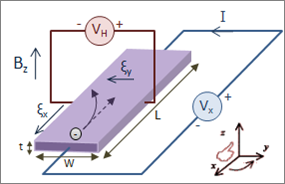
\includegraphics[scale=1]{figura_1.png}
\caption{\label{fig:epsart}Efecto Hall en un conductor con forma de placa.}
\end{figure}


\begin{equation}
\vec{F_L} = q\vec{E} + q\vec{v} \times \vec{B}
\end{equation}

Al campo eléctrico generado por $V_H$ es el campo de Hall $E_H$. Por Ley de Coulomb ésta produce una fuerza sobre
los electrones en sentido contrario a la fuerza producida por el campo magnético. Despues de un tiempo suficiente estas fuerzas
se equilibrarán y por tanto la fuerza de Lorentz de anulara, por lo que queda la siguiente ecuación

\begin{equation}
e\vec{E_H} = -e\vec{v} \times \vec{B}
\end{equation}

donde $e$ es la carga del electrón. Por otro lado se sabe que la magnitud del campo eléctrico entre dos placas paralelas
(la acumulación y déficit de electrones en caras opuestas del conductor) es

\begin{equation}
\vec{E_H} = \frac{\vec{V_H}}{w}
\end{equation}

donde $w$ es el ancho del conductor. La carga total $Q$ en el conductor es el número $n$ de cargas $q$ que pasan por el
volumen del conductor

\begin{equation}
Q = -newhL
\end{equation}

donde $h$ es la altura y $L$ el largo del conductor. La velocidad de los elctrones es $v = L/t$ y la corriente que pasa
por el conductor es $I = Q/t$, considerando el mismo tiempo en ambas expresiones se obtiene que

\begin{equation}
v = \frac{IL}{Q} = -\frac{IL}{ewh}.
\end{equation}

Tomando la magnitud de $E_H$ de la \textbf{Eq. 2} y sutituyendo la \textbf{Eq. 3} y la \textbf{Eq. 5} queda la siguiente expresión

\begin{equation}
V_H = -\frac{I B sen\theta}{n e h}
\end{equation}

donde $\theta$ es el ángulo entre $\vec{I}$ y $\vec{B}$. Siguiendo la \textbf{Fig. 1} consideramos $\theta = \pi/2$ y la ecuación
se reduce a

\begin{equation}
V_H = R_H \frac{I B}{h}
\end{equation}

donde se define $R_H$, la constante de Hall, como

\begin{equation}
R_H = -\frac{1}{ne}
\end{equation}

de donde es fácil ver que el signo de los portadores de carga determina el signo de la constante de Hall. También se nota el porque
es mejor utilizar semiconductores en los experimentos, pues al tener menos cantidad de cargas que se mueven, la constante
de Hall sera más grnade y por tanto será más fácil de medir, e inversamente al saber la magnitud de la constante de Hall
se puede estimar la cantidad portadores de la carga en el material.


%---------------------------------------------------------------------------
% METODOLOGY SECTION
%---------------------------------------------------------------------------

\section{Metodología}

Se realizarón varios experimentos para alcanzar los objetivos planteados. En todos los casos se utilizó una punta Hall de espesor $h = 0.15 mm$
de LnAs [2].

\subsection{Caracterización Electroimán}

Se trabajó con un electroimán de tipo herradura conectado a una fuente que le suministraba una corriente $I_E$. La fuente se econtraba
conectada en serie a un multimetro (Steren MUL-600) para medir la corriente suministrada.
Y con un gaussmetro (5180 Gauss/Tesla MeterFWBell) colocado lo mejor centrado en el electroimán, se fue midiendo el campo
magnético respecto a cambios de la corriente $I_E$ partiendo desde $0$ en saltos de apróximadamente $10\ mA$ hasta los $200\ mA$.

\subsection{ Caracterización de la Punta Hall a $I_C$ Constante}

De la \textbf{Eq. 7} se puede ver que hay dos formas de determinar $R_H$, dependiendo de que variables se conocen. En esta parte
del experimento se fija la corriente de control suministrada a la punta Hall. Y se varia el campo magnetico en intervalos de $50\ G$
para así obtener varias mediciones de $V_H$ y posteriormente poder hacer una ajuste de recta.

Para utilizar la punta Hall se conecta ésta a una caja de control que proporciona una corriente de control modulable (gracias a dos
pilas internas de 1.5 V) a la punta, y recibe el voltaje de Hall que experimenta la punta. Por lo que se conectan dos
multimetros (Steren MUL-600), uno que mide el voltaje y otro la corriente suministrada. La punta Hall se coloca en el
centro del electroimán de manera que la sus caras sean perpendiculares al campo magnético que es horizontal.  Se hacen 22
mediciones de $V_H$ para tres $I_C$ constantes.

\begin{figure}
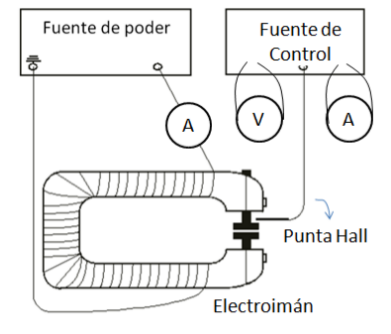
\includegraphics[scale=0.5]{figura_2.png}
\caption{\label{fig:epsart}Montaje general del experimento.}
\end{figure}


\begin{figure}
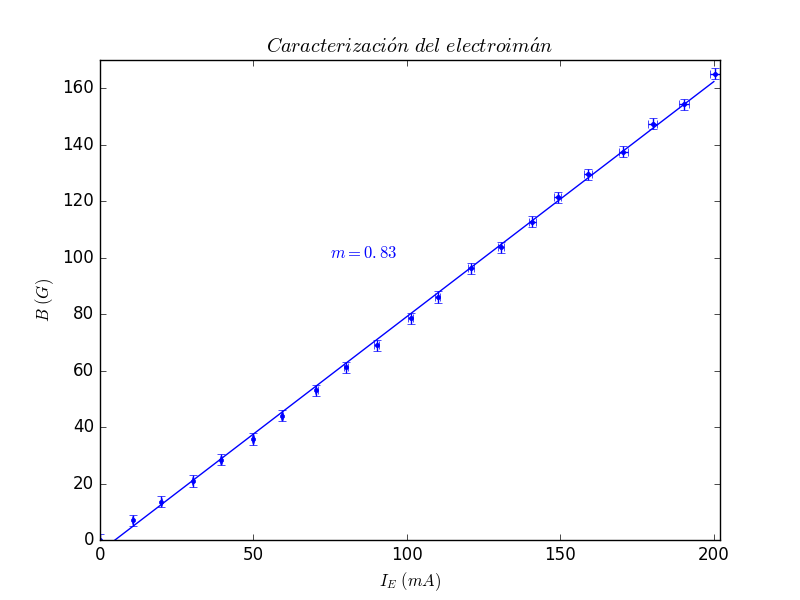
\includegraphics[scale=0.46]{figura_3.png}
\caption{\label{fig:epsart}Gráfica de las mediciones de $I_C$ vs $B$, y su ajuste de recta por mínimos cuadrados.}
\end{figure}

\begin{figure}
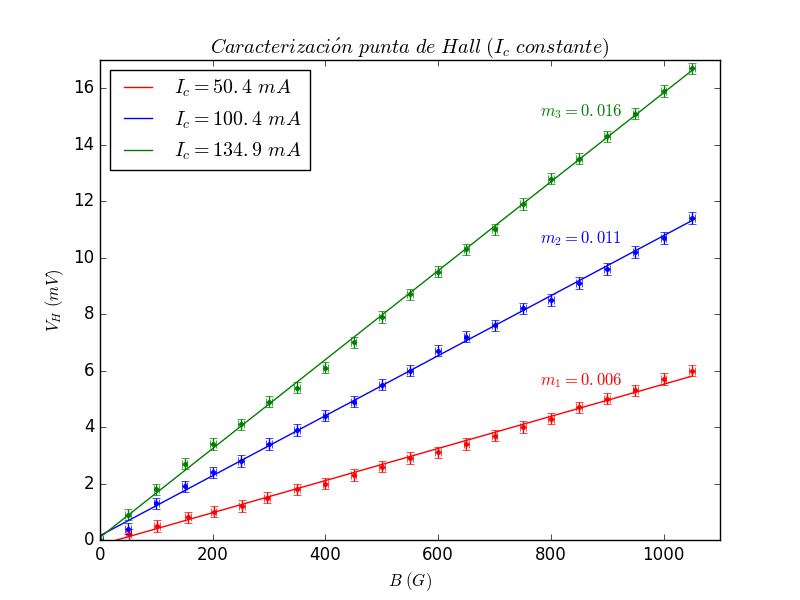
\includegraphics[scale=0.46]{figura_4.png}
\caption{\label{fig:epsart}Gráfica de los datos de $B$ vs $V_H$ para tres corrientes fijas distintas. Y sus respectivas rectas ajustadas
por mínimos cuadrados.}
\end{figure}

\subsection{Caracterización de la Punta Hall a $B$ Constante}

La configuración es exactamente la misma al caso anterior, sólo que ahora se fija el campo magnético del electroimán, y se varia
la corriente de control en intervalos de $10\ mA$, para así obtener $14$ mediciones de $V_H$ y se hace para tres valores de $B$ fijos.

\subsection{Variación de $V_H$ respecto al ángulo $\theta$}

En este caso se fija tanto la corriente de control $I_C$ como el campo $B$ durante las mediciones de $V_H$. Lo que se varia
es la posición de la punta Hall que inicialmente se encuetra con sus caras horixontales, y se va rotando $15^\circ$ en sentido de las
manecillas del reloj hasta que de una vuelta completa. De manera que se obtienen 24 mediciones y se repite el proceso para
tres campos $B$ distintos.

\subsection{Mapeo del Campo Magnético del Electroimán}

Se fija tanto la corriente de contro $I_c$ como el campo $B$ del electroimán, Entonces
se divide el electroimán en 100 regiones cuadradas de $1\ cm^2$, ya que las placas del electroimán son circulares con un radio
de $5\ cm$, esto se hace con ayuda de dos reglas. Siguiendo esta división se mide el el voltaje $V_H$ en cada región procurando
siempre colocar la punta en el centro de la placa y también lo mejor centrado de cada región. Despues se realiza un mapa de calor
con los datos obtenidos.

\subsection{Mapeo del campo de un Imán Permanente}

Análogamente al caso anterior se fijó un campo $B$ y una corriente de control $I_C$. Se utilizó un iman rectangular con
dimensiones de $15.1\ cm \times 10.3\ cm$ y se busco mapear su campo manético dividiendolo en zonas de
$1\ cm^2$ pues se dividio a lo largo (eje X) en intervalos de $1\ cm$ y a lo ancho (eje Y) también en intervalos de $1\ cm$. Se
midio el voltaje de Hall $V_H$ en cada región y se realizo el mismo procedimiento para tres alturas diferentes.


%---------------------------------------------------------------------------
% RESULTS SECTION
%---------------------------------------------------------------------------
\section{Análisis de Resultados}

\subsection{Caracterizacióm del Electroimán}

\begin{figure}
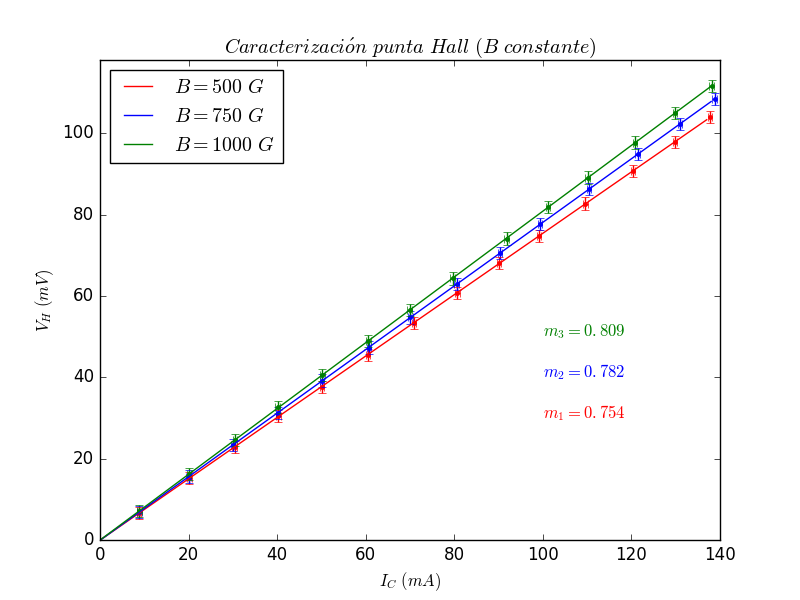
\includegraphics[scale=0.46]{figura_5.png}
\caption{\label{fig:epsart}Gráfica de los datos de $I_C$ vs $V_H$ para tres campos $B$ fijos distintos, y sus respectivos ajustes de recta
por mínimos cuadrados.}
\end{figure}


\begin{figure}
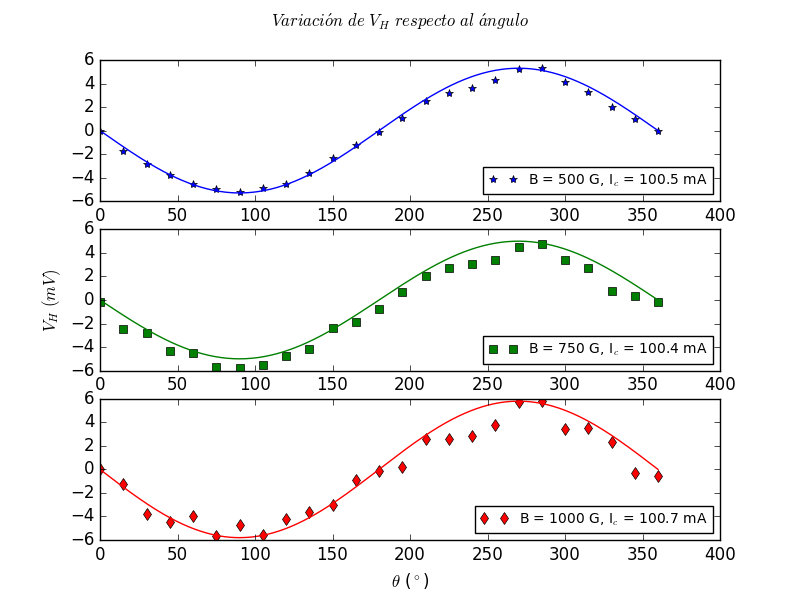
\includegraphics[scale=0.46]{figura_6.png}
\caption{\label{fig:epsart}Gráfica de las tres series de datos de $V_H$ cuando se rota la punta un ángulo $\theta$, para tres campos $B$
distintos. En cada apartado se incluye la gráfica de un $-sen(\theta)$ para encaja muy bien con los datos.}
\end{figure}


\begin{figure}
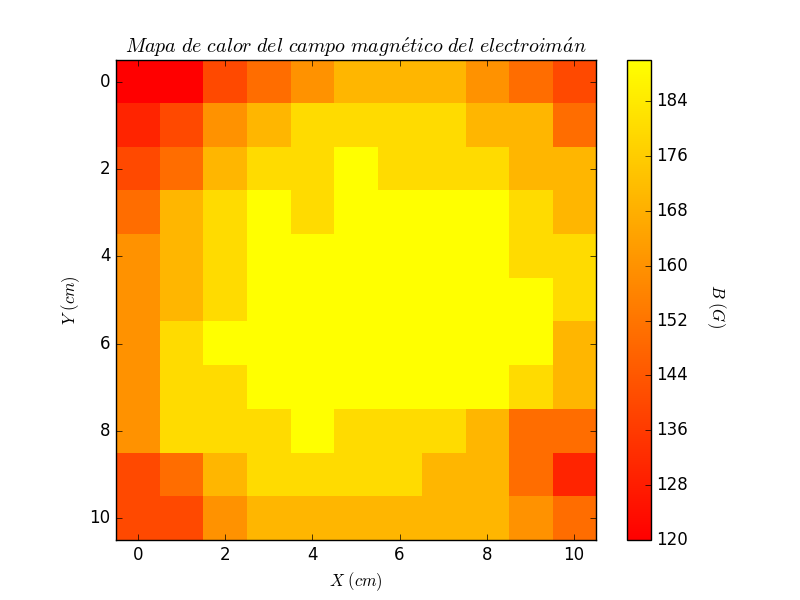
\includegraphics[scale=0.46]{figura_7.png}
\caption{\label{fig:epsart}Mapa de calor del campo magnético del electroimán medido en el centro, i.e, entre las dos placas.}
\end{figure}

\begin{figure}
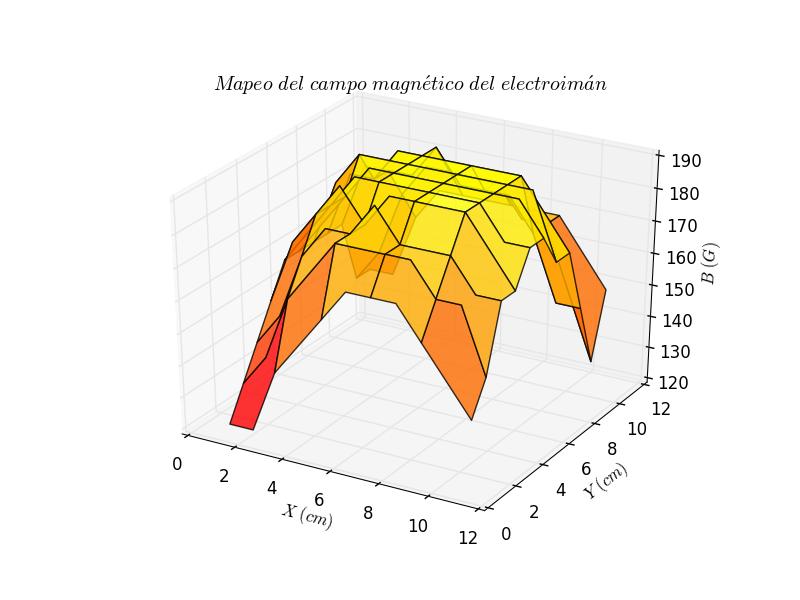
\includegraphics[scale=0.46]{figura_8.png}
\caption{\label{fig:epsart}Gráfica 3D del campo magnético del electroimán, donde el eje Z representa a $B$ y se observa de manera
más gráfica las zonas de más uniformidad e intensidad.}
\end{figure}

En la \textbf{Fig. 3} se puede ver que la relación entre la corriente eléctrica que se le suministraba al electroimán, con el
campo magnético que este proporcionaba, es lineal. De manera que utilizando el procedimiento de mínimios cuadrados, es posible
ajustar una recta, y obtener la constante de proporción entre $I_E$ y $B$ que es $m = 0.83$. De esta manerá será posible
saber con que campo magnético trabajamos con sólo conocer la corriente suministrada al electroimán.


\subsection{Caracterización de la punta Hall a $I_C$ constante}

Se realizarón tres series de medidas de $V_H$ (mV) para distintas corrientes de control $I_C$ y los resultados se muestran
en la \textbf{Fig. 4}, donde se puede apreciar un comportamiento lineal, como se esperba, por lo que ajustando una recta a cada
serie de puntos, se obtiene su pendiente y utilizando la \textbf{Eq. 7} es posible calcular la constante de Hall $R_H$ para
cada serie de puntos. Finalmente de estas se hace un promedio y se obtiene valor siguiente:

$$R_{HI_C} = (1.73 \pm 0.04)\times10^{-8} \frac{Vm}{AG}$$



\subsection{Caracterización de la punta Hall a $B$ constante}

De manera análoga al caso anterior, se realizarón tres series de medidas del voltaje $V_H$ para tres valores fijos distintos del
campo magnético $B$. En la \textbf{Fig. 5} se muestran los resultados y se observa nuevamente un comportamiento lineal, de
manera que al hacer el ajuste de recta y usando su correspondiente pendiente, junto con la \textbf{Eq. 7} se obtienen tres valores
de $R_H$ y su promedio es:

$$R_{HB} = (1.67 \pm 0.04)\times10^{-8} \frac{Vm}{AG}$$

comparando los valores de la constante de Hall $r_{HI_C}$ y $R_{HB}$ notamos que... por lo que para el analisís de las siguientes partes del
experimento el valor de la constante de Hall, se tomará el valor promedio de ambas:

$$R_H = (1.70 \pm 0.08)\times10^{-8} \frac{Vm}{AG}$$



Dado que $R_H$ tiene signo positivo de la \textbf{Eq. 8} podemos concluir que los portadores de la carga son los electrones, y por tanto
se trata de un semiconductor tipo n [3].

\subsection{Variación de $V_H$ respecto al ángulo $\theta$}


Se realizarón tres series de mediciones, todas para una corriente de control fija de alrededor de 100 mA, véase \textbf{Fig. 6}, y
tres valores de $B$ distintos, pero que se fijaban para su respectiva serie de mediciones. Se comenzó a medir $V_H$ con
la punta de Hall en posición horizontal, luego se iba rotando por intervalos de $15^\circ\ \pm 7.5^\circ$ que era la mínima escala del la
base graduada sobre la que se encontraba la punta Hall. En la \textbf{Fig. 6} se muestran los tres casos, en los cuales
es facilmente apreciable que tinen presente un comportamiento senoidal, como se esperaba por la presencia del factor $sin(\theta)$
en la \textbf{Eq. 6} debido a la naturaleza vectorial de la fuerzas implicadas en el efecto.

Este es un resultado importante por que muestra la importancia de alinear la punta Hall con el campo que medira, y como se verá más adelante
este aspecto tiene relevante importancial momento de mapear el campo magnético de un imán permanente.

\subsection{Mapeo del Campo Magnético del Eletroimán}

Tanto para las mediciones de esta sección como los de la siguiente, sobre el imán permanente, los valores del campo
se obtuvieron utilizando la \textbf{Eq. 7} dado que fijamos $I_C$ y midiendo $V_H$ podemos obtener $B$. Se fija
el campo del electroimán, y se realizan mediciones de $V_H$ en cada una de las regiones en las que se dividio el electroimán.
Cabe mencionar, que dado que la división se realizó colocando dos reglas en los ejes, las posiciones no son muy precisas, sin
embargo, se procuro en la mayor medida centrar lo meor posible la punta Hall.

En la \textbf{Fig. 7} se muestra un mapa de calor del valor del campo $B$. Mientras que en la \textbf{Fig. 8} se presentan los mismos
datos pero en una gráfica 3D, en la cual es más fácil de apreciar las zonas de mayor y menor intensidad del campo. Se nota
un área en el centro del electroimán con un campo más intenso y uniforme, esto es de esperarse dado que se trata de un
embobinado. Mientras que en las esquinas el valor del campo alcanza sus valores mas bajos, esto también es de esperarse
dado que las placas del electroimán son circulares y la region que se midio cuadrada, por lo que en esas zonas ya no esta la
cara del electroimán y el campo que se oberva se debe principalmente a los efectos de borde.


\subsection{Mapeo del Campo Magnético del Imán Permanente}

\begin{figure}
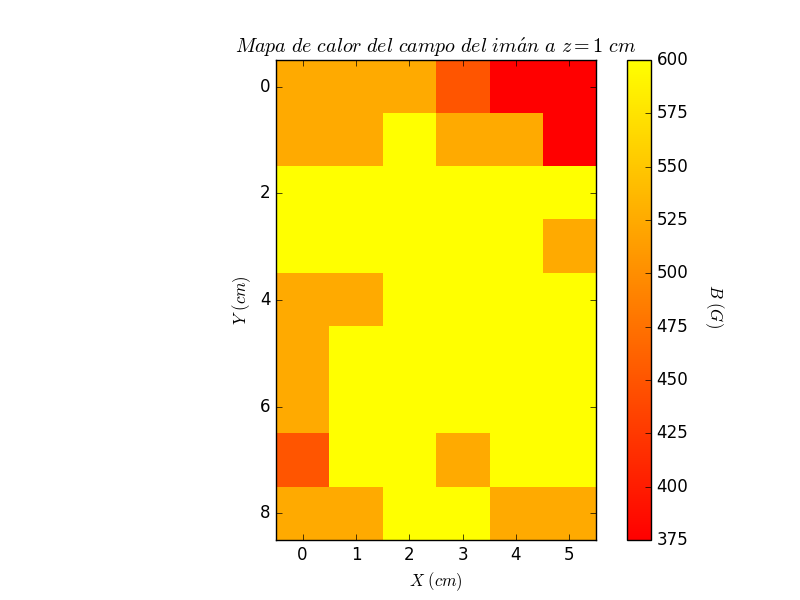
\includegraphics[scale=0.46]{figura_9.png}
\caption{\label{fig:epsart}Mapa de calor del campo magnético del imán permanente a una altura $z = 1\ cm$.}
\end{figure}

\begin{figure}
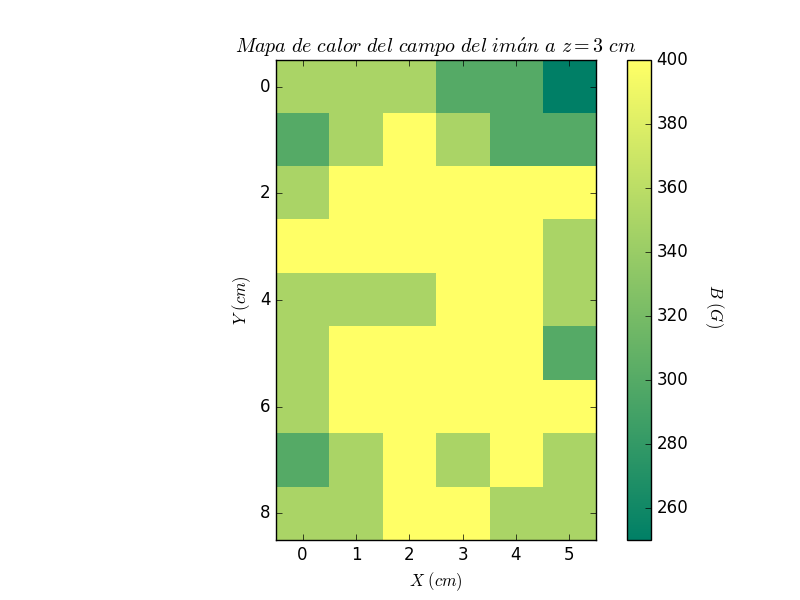
\includegraphics[scale=0.46]{figura_10.png}
\caption{\label{fig:epsart}Mapa de calor del campo magnético del imán permanente a una altura $z = 3\ cm$.}
\end{figure}

\begin{figure}
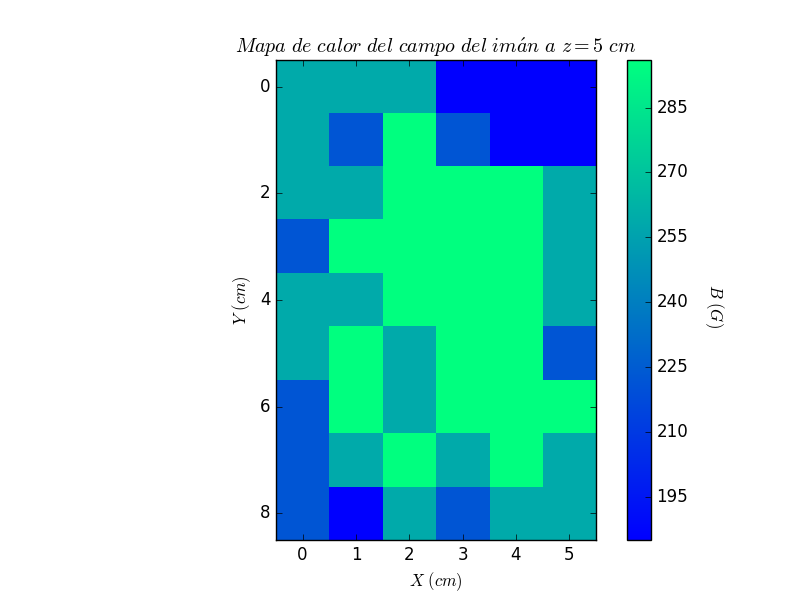
\includegraphics[scale=0.46]{figura_11.png}
\caption{\label{fig:epsart}Mapa de calor del campo magnético del imán permanente a una altura $z = 5\ cm$.}
\end{figure}

\begin{figure}
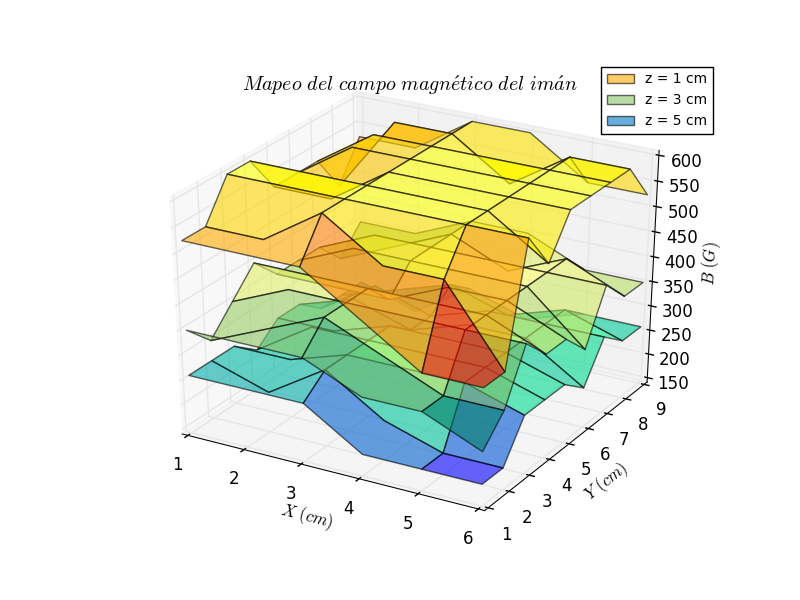
\includegraphics[scale=0.46]{figura_12.png}
\caption{\label{fig:epsart}Gráfica 3D de los tres mapeos del campo magnético del imán permanente, en la cual se pueden comparar
más fácilmente, se distinguen las zonas de uniformidad y las de mayor intensidad.}
\end{figure}

Se realiza una serie de mediciones análogas al caso anterior, solo difiriendo ahora la geometria del imán que es una barra, por
lo que se hacen más mediciones a lo largo que a lo ancho. Pero la verdadera novedad radíca en que se hacen tres de estos mapeos
para tres alturas distintas $1 \pm 0.5 cm$, $3 \pm 0.5 cm$ y $5 \pm 0.5 cm$. En \textbf{Fig. 9}, \textbf{Fig. 10} y \textbf{Fig. 11}, se
muestran los mapas individualmente de cada caso respectivamente. Mientras que en \textbf{Fig. 12} se juntan en una gráfica 3D
los tres mapeos para poder compararlos de mejor manera.

En primera intancia se nota que la intensidad del campo magnético, disminuye considerablemente conforme se va aumentando
la distancia en el eje Z. En los tres casos se observan dos zonas particulares, una al centro, que es donde se obtienen
las mediciones mas intensas, sin embargo, conforme la altura z va aumentando, esta región va disminuyendo su área. Esto se debe
a la forma conocida que tienen las líneas de campo magnético, yendo de un polo a otro, y como se observo en la \textbf{Sec. D}
el ángulo de la cara de la punta Hall respecto al campo $\vec{B}$ afecta considerablemente su medición. Entonces en las regiones más
cercanas al imán, las lineas de campo serán casi perpendiculares a este, por lo que las mediciones con la punta Hall, que se realizarón
con la punta de posición horizontal en todo momento, registrara una mayor intensidad del campo. Es por ésta misma geometría
de las líneas de campo, por la que el mapeo se complica considerablemente, pues a diferencia del electroimán donde se esperan lineas
másn uniforme en una dirección. Aqui las variaciones, no solo dependen del campo sino la forma de medirlo.

Pese a todo esto,
los resultados de la \textbf{Fig. 12} son suficientes para mostrar lo que esperabamos. La otra región interesante, que se
presenta en las tres alturas es la de la esquina superior derechas, pues allí se alcanzan los valores más pequeños del campo.
Esto se atribuye a que la barra en esa parte se encontraba despostillada considerablemente, lo que da lugar a que las lineas del
campo tengan un comportamiento más complicado y genere mediciones como las mostradas. En general el contorno del imán se
encontraba bastante golpeado, por lo que intentar tomar mediciones en esas zonas arrojaria resultados imprevisibles. Es por
eso que las mediciones se enfocarón en una zona rectangular de menor tamaño al del imán, donde se esperaba que las lineas
de campo tuvierán un comportamiento más parecido al esperado.



%---------------------------------------------------------------------------
% CONCLUSIONS SECTION
%---------------------------------------------------------------------------
\section{Conclusiones}

Se realizo el principal objetivo de determinar el valor de $R_H = (1.70 \pm 0.08)\times10^{-8} \frac{Vm}{AG}$ para una punta
Hall y con ello se logro hacer mediciones del campo magnético para ver el comportamiento senoidal de $V_H$ cuando el campo
$B$ no es perpendicular a la corriente $I_C$ y finalmente se consiguio hacer un mapeo tanto del electroimán, en que se obervó
un comportamiento con simetría círcular, como se esperaba. Mientras que respecto al imán permanente en barra, el comportamiento
del campo magnético se observó más complicado, sin embargo, se consiguió apreciar las características cualitativas de este, como
son las zonas de mayor uniformidad al centro, y la disminución del campo con la altura. Todo usando la punta Hall como gaussmetro.

Para próximas reproducciones del experimento se recomienda, una mayor toma de datos en la \textbf{Sec. III.B} y la \textbf{Sec. III.C}
para obtener un mejor promedio, pero también se recomienda que siempre se realicen ambos procedimientos.
Mientras que para la \textbf{Sec. III.D}, aunque los resultados son muy buenos, se recomendaría utilizar una graduación de menor escala
a la utilizada($15^\circ$) para una menor incertidumbre y mayor cantidad de datos.

%---------------------------------------------------------------------------
% ACKNOWLEDGE SECTION
%---------------------------------------------------------------------------
\begin{thebibliography}{101}

\bibitem{1} G. B. Armen, Hall Effect Experiment (Notes online, 2007).
\bibitem{2} Manual de práctica ``Efecto Hall'', Facultad de Ciencias, UNAM, Laboratorio de Física Contemporánea II.
\bibitem{3} https://es.wikipedia.org/wiki/Semiconductor
\bibitem{4} Purcell, E. M., Electricity and Magnetism, Berkeley Physics Course Vol. 2, Third Edition.



\end{thebibliography}

%------------------------------ End Document ------------------------------
\end{document}

